\subsubsection{Scan Pattern}

The \definition{Scan Pattern} is used to \textbf{compute all partial results of an input sequence using a binary associative operation}. It generates a new sequence where each element is the result of applying the operation to all preceding elements in the input sequence.

\highspace
\begin{flushleft}
    \textcolor{Green3}{\faIcon{stream} \textbf{Types of Scans}}
\end{flushleft}
\begin{itemize}
    \item \definition{Inclusive Scan Pattern}
    \begin{itemize}
        \item[\textcolor{Red2}{\faIcon{book}}] \textcolor{Red2}{\textbf{Definition}}. Each element in the result sequence includes the value of the current element in the input sequence.
    
        \item[\textcolor{Green3}{\faIcon{poll}}] \textcolor{Green3}{\textbf{Result}}. The \textbf{result for each position is the combination} (using the associative operation) \textbf{of all elements up to and including the current element}.

        \item[\textcolor{Green3}{\faIcon{check-circle}}] \textcolor{Green3}{\textbf{Use Case}}. It is useful when the result must contain the current element at every position. It can be used in parallel algorithms where each step depends on all previous steps, including the current one.
    \end{itemize}
    \begin{examplebox}[: Inclusive Scan Pattern]
        For an input array \texttt{[A, B, C, D]}, an inclusive scan with an associative operation \texttt{+} results in:
        \begin{equation*}
            \texttt{[A, A + B, A + B + C, A + B + C + D]}
        \end{equation*}
        For numbers:
        \begin{itemize}
            \item Input: $\left[1, 2, 3, 4\right]$
            \item Output: $\left[1, 3, 6, 10\right]$
        \end{itemize}
    \end{examplebox}


    \item \definition{Exclusive Scan Pattern}
    \begin{itemize}
        \item[\textcolor{Red2}{\faIcon{book}}] \textcolor{Red2}{\textbf{Definition}}. Each element in the result sequence excludes the value of the current element from the input sequence. Instead, it includes the combination of all prior elements.
    
        \item[\textcolor{Green3}{\faIcon{poll}}] \textcolor{Green3}{\textbf{Result}}. The \textbf{result for each position is the combination} (using the associative operation) \textbf{of all elements before the current element}.

        \item[\textcolor{Green3}{\faIcon{check-circle}}] \textcolor{Green3}{\textbf{Use Case}}. It is useful for scenarios where the result at each position should exclude the current element and provide the cumulative effect of all previous elements. It's often used in algorithms that require a shift in position, such as calculating running sums starting from the next element.
    \end{itemize}
    \begin{examplebox}[: Exclusive Scan Pattern]
        For an input array \texttt{[A, B, C, D]}, an exclusive scan with an associative operation \texttt{+} results in:
        \begin{equation*}
            \texttt{[$\times$, A, A + B, A + B + C]}
        \end{equation*}
        Where $\times$ is the identity element of the operation. For numbers:
        \begin{itemize}
            \item Input: $\left[1, 2, 3, 4\right]$
            \item Output: $\left[0, (1), (1 + 2), (1 + 2 + 3)\right] = \left[0, 1, 3, 6\right]$
        \end{itemize}
    \end{examplebox}
\end{itemize}

\highspace
\begin{flushleft}
    \textcolor{Green3}{\faIcon{tachometer-alt} \textbf{Techniques for parallelizing Scan Pattern}}
\end{flushleft}
\begin{itemize}
    \item \definition{Prefix Maximum Algorithm with Up and Down Sweep}
    \begin{itemize}
        \item[\textcolor{Red2}{\faIcon{book}}] \textcolor{Red2}{\textbf{Definition}}. Prefix Maximum Algorithm with Up and Down Sweep is a special \textbf{implementation of the scan pattern}, \textbf{designed to find the maximum value within an array using parallel processing}.
        
        \highspace
        It \hl{calculates the maximum value at the \emph{i}-th index of the input array} and contains the \hl{maximum value of the array at the last position}.

        \highspace
        For \example{example}, given the array:
        \begin{equation*}
            \texttt{[1, 4, 0, 2, 7, 2, 4, 3]}
        \end{equation*}
        It returns:
        \begin{equation*}
            \texttt{[1, 4, 4, 4, 7, 7, 7, 7]}
        \end{equation*}
        Where indicates that at position 2, the sub-array \texttt{[1, 4, 0]}, the maximum value that can be found is \texttt{4}.

        \highspace
        It consists of two main phases: Up-Sweep (Reduce) Phase and Down-Sweep Phase.

        \item[\textcolor{Green3}{\faIcon{tools}}] \textcolor{Green3}{\textbf{Algorithm}}
        \begin{enumerate}
            \item \definitionWithSpecificIndex{Up-Sweep (Reduce) Phase}{Up-Sweep (Reduce)}{} \definition{}. Create a balanced binary tree of partial results, focusing on \textbf{finding the maximum value}.
            \begin{enumerate}
                \item \textbf{Pairwise Combination}: Begin by \hl{combining elements in pairs to find the maximum of each pair}.
                \item \textbf{Level-by-Level Combination}: Continue \hl{combining results at each level of the tree until a single result} (the maximum value) \hl{is obtained}.
            \end{enumerate}
            \begin{examplebox}[: Up-Sweep (Reduce) technique]
                We follow a tree approach to manually compute the up-sweep. We divide the input into pairs and evaluate each pair with the max operator. The result is the next node.

                \hqlabel{example: Up-Sweep (Reduce) technique}{For an array \texttt{[1, 4, 0, 2, 7, 2, 4, 3]}:}

                \begin{center}
                    \begin{tikzpicture}
                        [level distance=12mm,
                         level 1/.style={sibling distance=40mm},
                         level 2/.style={sibling distance=20mm},
                         level 3/.style={sibling distance=10mm},
                         every node/.style={draw, circle, inner sep=3pt},
                         edge from parent/.style={draw, {Stealth}-}]

                        \node {7} % Root
                        child {node {4}
                            child {node {4}
                            child {node {1} }
                            child {node {4} }
                            }
                            child {node {2}
                            child {node {0} }
                            child {node {2} }
                            }
                        }
                        child {node {7}
                            child {node {7}
                            child {node {7} }
                            child {node {2} }
                            }
                            child {node {4}
                            child {node {4} }
                            child {node {3} }
                            }
                        };
                    \end{tikzpicture}
                \end{center}
                The comparison made are:
                \begin{enumerate}
                    \item Level 1:
                    \begin{itemize}
                        \item Pairs:
                        \begin{itemize}
                            \item \texttt{max(1, 4)}
                            \item \texttt{max(0, 2)}
                            \item \texttt{max(7, 2)}
                            \item \texttt{max(4, 3)}
                        \end{itemize}
                        \item Result: \texttt{[4, 2, 7, 4]}
                    \end{itemize}

                    \item Level 2:
                    \begin{itemize}
                        \item Pairs:
                        \begin{itemize}
                            \item \texttt{max(4, 2)}
                            \item \texttt{max(7, 4)}
                        \end{itemize}
                        \item Result: \texttt{[4, 7]}
                    \end{itemize}

                    \item Level 3:
                    \begin{itemize}
                        \item Pair: \texttt{max(4, 7)}
                        \item Result: \texttt{[7]}
                    \end{itemize}
                \end{enumerate}
                At this point, the Up-Sweep phase has found the maximum value of the entire array.
            \end{examplebox}

            \item \definitionWithSpecificIndex{Down-Sweep Phase}{Down-Sweep}{}. Use the partial results from the Up-Sweep phase to \textbf{compute the final scan results for all elements in the array}.
            \begin{enumerate}
                \item \textbf{Initialization}: \hl{Begin with an initial value, typically the identity element} (for maximum, it could be negative infinity $-\infty$).
                \item \textbf{Propagate Results}: \hl{Propagate the maximum values back down the tree}, updating the results for each element.
            \end{enumerate}
            \setcounter{example}{36}
            \begin{examplebox}[ (continue): Down-Sweep technique]
                Continuing from the Up-Sweep phase result \texttt{[7]} and the original array \texttt{[1, 4, 0, 2, 7, 2, 4, 3]} (page \hqpageref{example: Up-Sweep (Reduce) technique}).
                
                \highspace
                The main rule followed during the down-sweep technique is the following: the left leaf always inserts the value of the parent node, while the right leaf inserts the value calculated after applying the \texttt{max} operation to the value of the parent node and the left side just removed (which we find on the up-sweep graph).
                
                \highspace
                On the last level of the tree, there is an exception: before inserting the left leaf directly, the \texttt{max} operation of the inherited value and the input value must be performed.

                \highspace
                The steps are detailed:
                \begin{enumerate}
                    \item Replace the maximum value on the root (\texttt{7}) and insert the identity element, in our case the $-\infty$.
                    \begin{center}
                        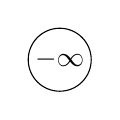
\begin{tikzpicture}
                            [level distance=14mm,
                             level 1/.style={sibling distance=40mm},
                             level 2/.style={sibling distance=20mm},
                             level 3/.style={sibling distance=10mm},
                             every node/.style={draw, circle, minimum size=8mm, inner sep=0pt},
                             edge from parent/.style={draw, -{Stealth}}]
    
                            \node {$-\infty$};
                        \end{tikzpicture}
                    \end{center}
                    \item Level 1:
                    \begin{itemize}
                        \item Insert the parent node on the left leaf, so $-\infty$.
                        \item On the right leaf, insert the performed operation between the parent's value and the left leaf of the up-sweep tree. So the values to compare are $-\infty$ and $4$: \texttt{max($-\infty$, 4) = 4}
                    \end{itemize}
                    \begin{center}
                        \begin{tikzpicture}
                            [level distance=12mm,
                             level 1/.style={sibling distance=20mm},
                             every node/.style={draw, circle, minimum size=8mm, inner sep=0pt},
                             edge from parent/.style={draw, -{Stealth}}]
    
                            \node {$-\infty$} % Root
                            child {node {$-\infty$}}
                            child {node {4}};
                        \end{tikzpicture}
                    \end{center}
                    \newpage
                    \item Level 2 ((from left to the right)):
                    \begin{itemize}
                        \item Vertex $-\infty$:
                        \begin{itemize}
                            \item Insert the parent node on the \textbf{left leaf}, so $-\infty$. It's not the last leaf of the tree, so we don't do any checking.

                            \item The \textbf{right leaf} comparison is between $-\infty$ (the father's value) and the left leaf on the up-sweep tree (the value just replaced by the $-\infty$), so 4. Again, the comparison is:
                            \begin{equation*}
                                \texttt{max($-\infty$, 4) = 4}
                            \end{equation*}
                        \end{itemize}

                        \item Vertex $4$:
                        \begin{itemize}
                            \item Insert the parent node on the \textbf{left leaf}, so $4$.
                            \item The \textbf{right leaf} comparison is between 4 (the father's value) and the left leaf on the up-sweep tree (the value just replaced by 4), so 7. The comparison is:
                            \begin{equation*}
                                \texttt{max(4, 7) = 7}
                            \end{equation*}
                        \end{itemize}
                    \end{itemize}
                    \begin{center}
                        \begin{tikzpicture}
                            [level distance=14mm,
                             level 1/.style={sibling distance=40mm},
                             level 2/.style={sibling distance=20mm},
                             level 3/.style={sibling distance=10mm},
                             every node/.style={draw, circle, minimum size=8mm, inner sep=0pt},
                             edge from parent/.style={draw, -{Stealth}}]
    
                            \node {$-\infty$} % Root
                            child {node {$-\infty$}
                                child {node {$-\infty$}}
                                child {node {4}}
                            }
                            child {node {4}
                                child {node {4}}
                                child {node {7}}
                            };
                        \end{tikzpicture}
                    \end{center}
                    \item Level 3 (from left to the right):
                    \begin{itemize}
                        \item Vertex $-\infty$:
                        \begin{itemize}
                            \item \textbf{Left leaf}. Since this is the last level, we need to compute an extra check. We need to compute:
                            \begin{equation}
                                \texttt{max(inherited val, input val)}
                            \end{equation}\label{eq: down-sweep last level}
                            In our case, the inherited value is the $-\infty$, but the input value on the first position is 1. Therefore:
                            \begin{equation*}
                                \texttt{max($-\infty$, 1) = 1}
                            \end{equation*}
                            \item \textbf{Right leaf}. We compare the value we just removed, 1, to the value of the parent: $-\infty$.
                            \begin{equation*}
                                \texttt{max(1, $-\infty$) = 1}
                            \end{equation*}
                            The result should be 1 \underline{BUT} we are at the last level of the tree. So we need to do an extra check between the inherited value (what we want to place) and the input value on the second position (our case 4):
                            \begin{equation*}
                                \texttt{max(1, 4) = 4}
                            \end{equation*}
                        \end{itemize}
                        \item Vertex $4$:
                        \begin{itemize}
                            \item \textbf{Left leaf}. We apply formula \ref{eq: down-sweep last level} on page \pageref{eq: down-sweep last level}, the idea is the same as before:
                            \begin{equation*}
                                \texttt{max(4, 0) = 4}
                            \end{equation*}
                            \item \textbf{Right leaf}. We compare the value just removed, 0, to the value of parent: 4.
                            \begin{equation*}
                                \texttt{max(0, 4) = 4}
                            \end{equation*}
                            And the value obtained with the input value on the array:
                            \begin{equation*}
                                \texttt{max(4, 2) = 4}
                            \end{equation*}
                        \end{itemize}
                        \item Vertex $4$:
                        \begin{itemize}
                            \item \textbf{Left leaf}. We apply formula \ref{eq: down-sweep last level} on page \pageref{eq: down-sweep last level}, the idea is the same as before:
                            \begin{equation*}
                                \texttt{max(4, 7) = 7}
                            \end{equation*}
                            \item \textbf{Right leaf}. We compare the value just removed, 7, to the value of parent: 4.
                            \begin{equation*}
                                \texttt{max(7, 4) = 7}
                            \end{equation*}
                            And the value obtained with the input value on the array:
                            \begin{equation*}
                                \texttt{max(7, 2) = 7}
                            \end{equation*}
                        \end{itemize}
                        \newpage
                        \item Vertex $7$:
                        \begin{itemize}
                            \item \textbf{Left leaf}. We apply formula \ref{eq: down-sweep last level} on page \pageref{eq: down-sweep last level}, the idea is the same as before:
                            \begin{equation*}
                                \texttt{max(7, 4) = 7}
                            \end{equation*}
                            \item \textbf{Right leaf}. We compare the value just removed, 4, to the value of parent: 7.
                            \begin{equation*}
                                \texttt{max(4, 7) = 7}
                            \end{equation*}
                            And the value obtained with the input value on the array:
                            \begin{equation*}
                                \texttt{max(7, 3) = 7}
                            \end{equation*}
                        \end{itemize}
                    \end{itemize}
                    \begin{center}
                        \begin{tikzpicture}
                            [level distance=14mm,
                             level 1/.style={sibling distance=40mm},
                             level 2/.style={sibling distance=20mm},
                             level 3/.style={sibling distance=10mm},
                             every node/.style={draw, circle, minimum size=8mm, inner sep=0pt},
                             edge from parent/.style={draw, -{Stealth}}]
    
                            \node {$-\infty$} % Root
                            child {node {$-\infty$}
                                child {node {$-\infty$}
                                child {node {1} }
                                child {node {4} }
                                }
                                child {node {4}
                                child {node {4} }
                                child {node {4} }
                                }
                            }
                            child {node {4}
                                child {node {4}
                                child {node {7} }
                                child {node {7} }
                                }
                                child {node {7}
                                child {node {7} }
                                child {node {7} }
                                }
                            };
                        \end{tikzpicture}
                    \end{center}
                \end{enumerate}
            \end{examplebox}
        \end{enumerate}
    \end{itemize}
    \begin{figure}[!htp]
        \centering
        \includegraphics[width=.85\textwidth]{img/maximum-up-down-sweep-1.pdf}
        \caption{Graphical example of the Maximum Algorithm with Up and Down Sweep. On the left a sequential version and on the right a parallel version. The parallel version was analyzed on the previous pages.}
    \end{figure}


    \item \definition{Three-Phase Scan with Tiling}
    \begin{itemize}
        \item[\textcolor{Red2}{\faIcon{book}}] \textcolor{Red2}{\textbf{Definition}}. Three-Phase Scan with Tiling is a technique that \textbf{divides the input array into smaller tiles and processes them in three distinct phases} to efficiently perform the scan operation.
        
        The main goal is to improve parallelism and cache efficiency by splitting the input array into smaller tiles and processing them independently.

        \item[\textcolor{Green3}{\faIcon{tools}}] \textcolor{Green3}{\textbf{Algorithm}}
        \begin{enumerate}
            \item \definition{Tiling and Local Scan}. Divide the input array into smaller tiles and perform the scan operation on each tile independently.
            \begin{enumerate}
                \item \textbf{Divide the Input Array}: Break the input array into smaller blocks or tiles.
                \item \textbf{Local Scan} (Inclusive): Compute the scan for each tile independently.
            \end{enumerate}
            \begin{examplebox}[: Tiling and Local Scan]
                For an array \texttt{[1, 2, 3, 4, 5, 6, 7, 8]} with a tile size of 4:
                \begin{itemize}
                    \item Tiles: \texttt{[1, 2, 3, 4]} and \texttt{[5, 6, 7, 8]}
                    \item Local Scans:
                    \begin{itemize}
                        \item First tile: \texttt{[1, 3, 6, 10]}
                        \item Second tile: \texttt{[5, 11, 18, 26]}
                    \end{itemize}
                \end{itemize}
            \end{examplebox}

            \item \definition{Scan of Tile Results}. Compute the \textbf{scan of the final elements of each tile to handle dependencies between tiles}.
            \begin{enumerate}
                \item \textbf{Extract Final Elements}: Take the last element of each tile.
                \item \textbf{Global Scan}: Perform a scan operation on these final elements to propagate the results across tiles.
            \end{enumerate}
            \begin{examplebox}[: Scan of Tile Results]
                \begin{itemize}
                    \item Final Elements: \texttt{10} (from the first tile) and \texttt{26} (from the second tile)
                    \item Global Scan: \texttt{[10, 36]} (assuming addition and identity element \texttt{0})
                \end{itemize}
            \end{examplebox}

            \item \definition{Distribution of Tile Results}. \textbf{Distribute the results of the scanned tile results to all elements in their respective tiles}.
            \begin{enumerate}
                \item \textbf{Distribute Results}: Add the scan results of the previous tiles to the elements of the current tile.
            \end{enumerate}
            \begin{examplebox}[: Distribution of Tile Results]
                \begin{itemize}
                    \item First Tile Remains the Same: \texttt{[1, 3, 6, 10]}
                    \item Second Tile: add the scan result \texttt{10} from the first tile's last element:
                    \begin{itemize}
                        \item \texttt{5 + 10 = 15}
                        \item \texttt{11 + 10 = 21}
                        \item \texttt{18 + 10 = 28}
                        \item \texttt{26 + 10 = 36}
                    \end{itemize}
                    \begin{equation*}
                        \texttt{[15, 21, 28, 36]}
                    \end{equation*}
                \end{itemize}
                Combining the results of the two tiles, we get:
                \begin{equation*}
                    \texttt{[1, 3, 6, 10, 15, 21, 28, 36]}
                \end{equation*}
            \end{examplebox}
        \end{enumerate}
    \end{itemize}
    \begin{figure}[!htp]
        \centering
        \includegraphics[width=\textwidth]{img/three-phase-scan-with-tiling-1.pdf}
        \caption{Graphical example of the Three-Phase Scan with Tiling.}
    \end{figure}


    \item \definition{Fusion of Map Pattern with Scan Pattern}
    \begin{itemize}
        \item[\textcolor{Red2}{\faIcon{book}}] \textcolor{Red2}{\textbf{Definition}}. Combine the transformation capabilities of the map pattern with the cumulative operations of the scan pattern to \textbf{achieve more complex and efficient parallel computations}.
        
        When we fuse the map and scan patterns, we \textbf{first apply the map function to transform each element in the input sequence}, and \textbf{then apply the scan operation to the transformed sequence}.

        \item[\textcolor{Green3}{\faIcon{tools}}] \textcolor{Green3}{\textbf{Algorithm}}
        \begin{enumerate}
            \item \textbf{Apply Map Function}: Transform each element in the input sequence using the map function.
            \item \textbf{Apply Scan Operation}: Perform the scan operation on the transformed sequence to compute cumulative results.
        \end{enumerate}
    \end{itemize}
    \begin{examplebox}[: Fusion of Map Pattern with Scan Pattern]
        Let's consider a practical example where we want to compute the prefix sums of the squares of an input array \texttt{[1, 2, 3, 4]}.
        \begin{enumerate}
            \item \textbf{Map Function}
            \begin{enumerate}
                \item Define the map function as $f\left(x\right) = x^{2}$.
                \item Apply the map function: \texttt{[1, 4, 9, 16]} (squares of the input elements),
            \end{enumerate}
            \item \textbf{Scan Operation}
            \begin{enumerate}
                \item Perform an inclusive scan on the transformed sequence \texttt{[1, 4, 9, 16]}.
                \item Inclusive scan result: \texttt{[1, 5, 14, 30]}.
            \end{enumerate}
        \end{enumerate}
    \end{examplebox}
    \begin{figure}[!htp]
        \centering
        \includegraphics[width=\textwidth]{img/fusion-map-with-scan-1.pdf}
        \caption{Graphical example of the Fusion of Map Pattern with Scan Pattern.}
    \end{figure}
\end{itemize}
